\documentclass[a4paper,10pt,titlepage]{article}

\usepackage[utf8]{inputenc}
\usepackage[czech]{babel} % francais, polish, spanish, ...
\usepackage[T1]{fontenc}

\usepackage{lmodern} % Type1-font for non-english texts and characters
\usepackage{enumitem} % enumerations
\usepackage{graphicx} % images
\usepackage{float}

\graphicspath{ {images/} }

\title{Vývoj informačních systémů\\Informační systém pro střední školy} % název
\author{Jakub Beránek} % autor
\date{2015} %datum

\begin{document}
  \maketitle

	\section{Vize}
	Tento dokument popisuje informační systém pro střední školy, který bude sloužit k evidenci informací o studiu.
	Tento systém je potřebný pro zefektivnění komunikace mezi studenty a učiteli, zajištění centrální správy
	údajů o studiu a zajištění rychlého přístupu k těmto údajům.
	Využívat ho budou učitelé a studenti, pro obě dvě skupiny bude systém poskytovat odlišnou sadu funkcí.
	O správu účtů a konfiguraci celého systému se budou starat administrátoři.
	
	\vspace{5mm} %5mm vertical space
	
	Učitelům bude nabízet správu známek studentů, zadávání jejich absence, přidávání upozornění na blížící se testy a úpravu rozvrhů.
	Studentům bude systém zobrazovat jejich známky, počítat jejich průměry, vypočítávat a upozorňovat na absenci v předmětech,
	zobrazovat rozvrh, suplování a testy zadané učiteli. Administrátoři budou mít možnost spravovat uživatelské účty, předměty, třídy a konfigurovat
	celý systém.
	
	\vspace{5mm} %5mm vertical space
	
	Aplikace bude běžet na serveru školy, uživatelé k ní budou moci přistupovat přes webové rozhraní a mobilní aplikaci.
	Jelikož je potřeba, aby učitelé mohli zadávat známky a testy bez omezení a studenti jej budou využívat dennodenně k získání
	aktuálních informací o studiu, aplikace bude dostupná neustále.
	
	\section{Funkční specifikace}
	\subsection{Use case model}
		\begin{figure}[h!]
			\centering
					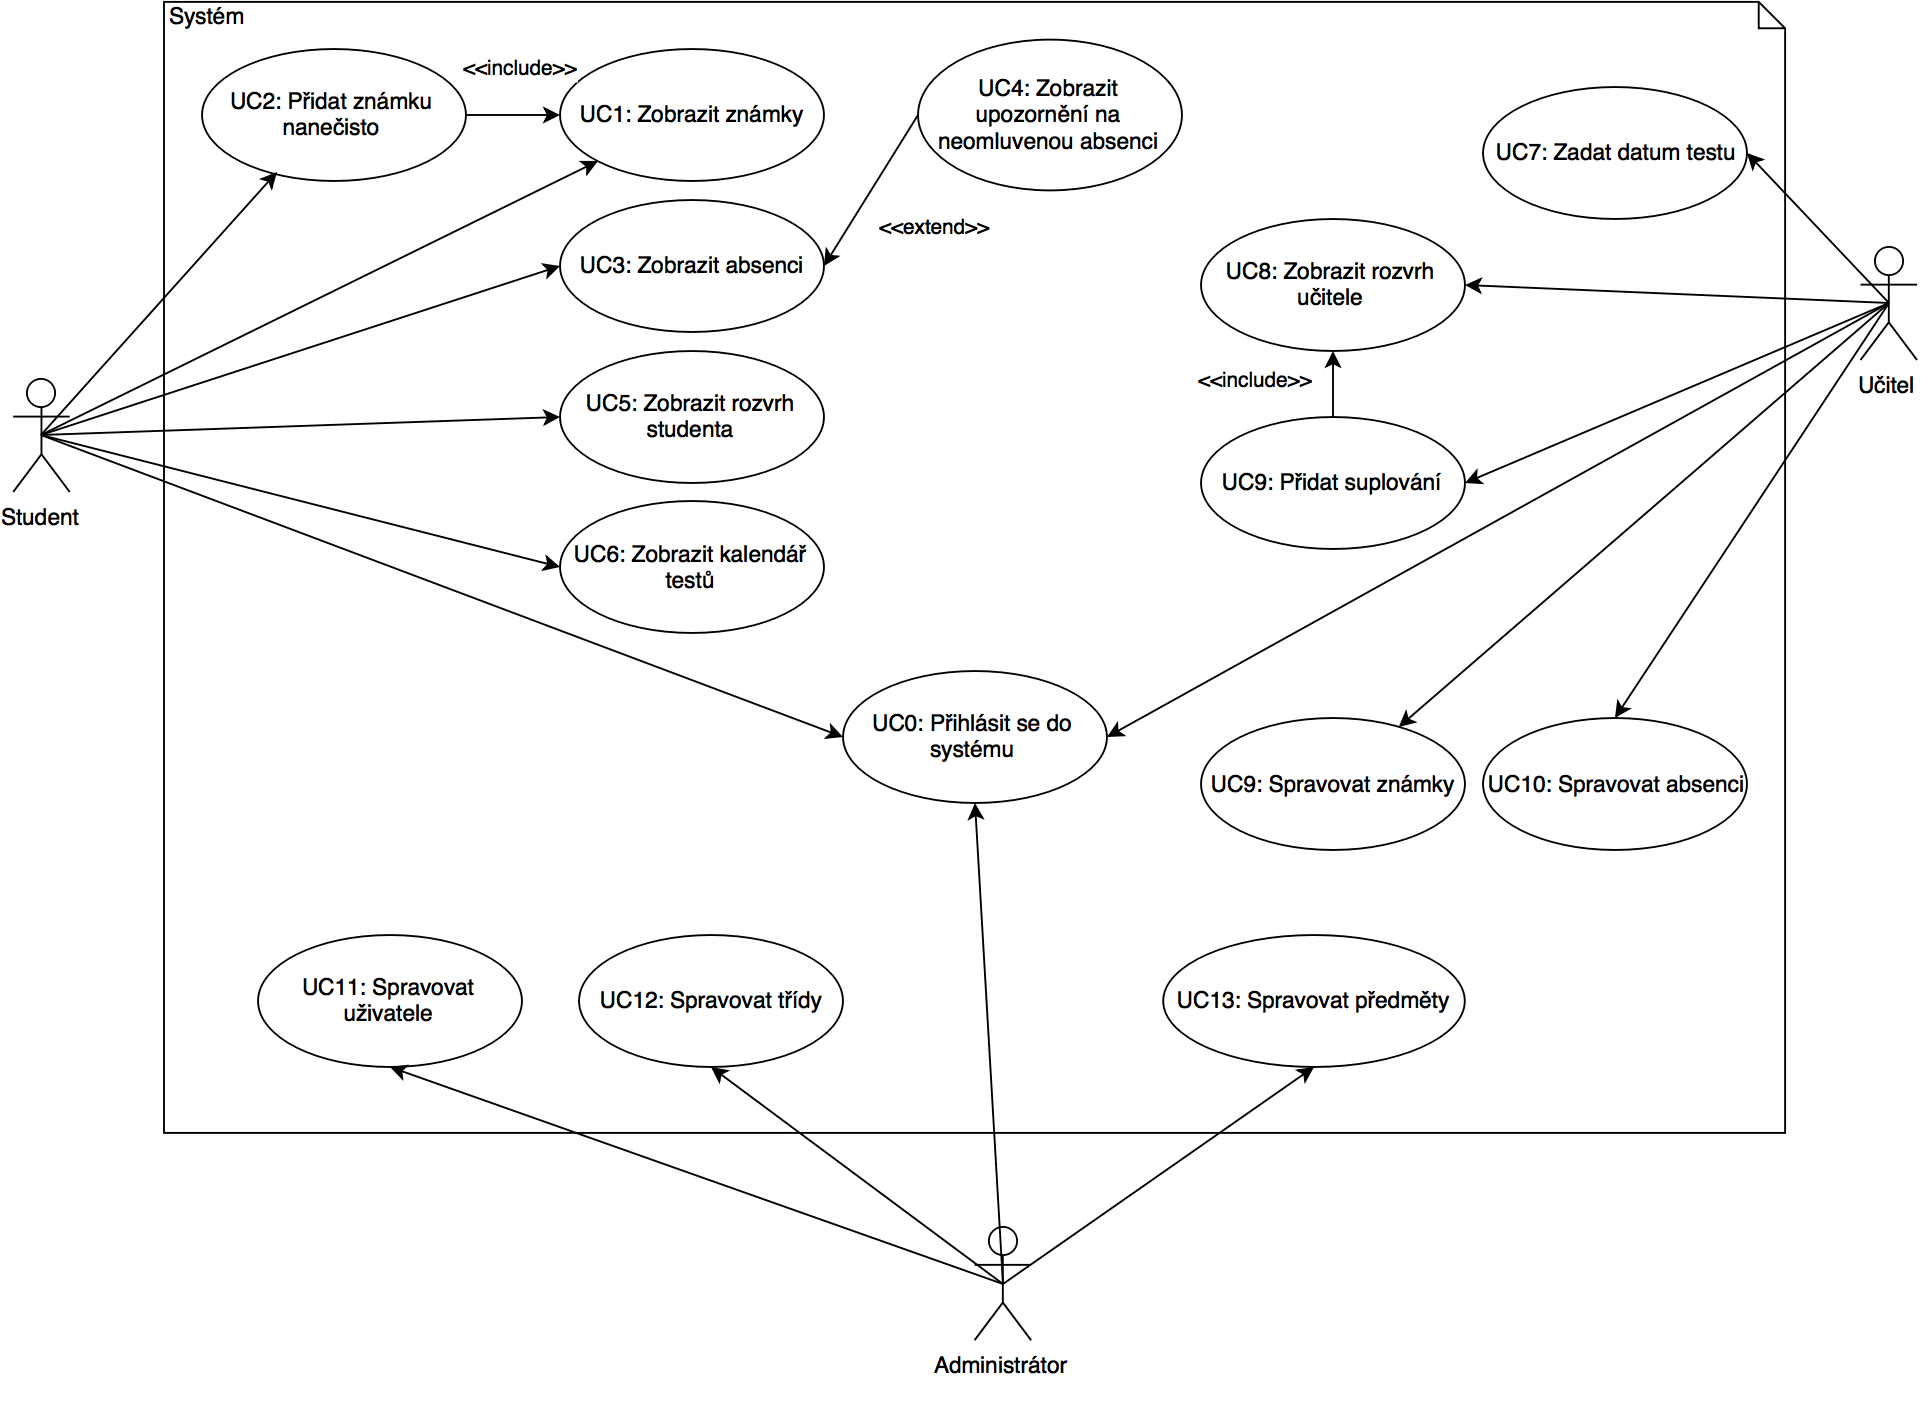
\includegraphics[width=\textwidth]{vis_use_case_diagram}
			\caption{Use case diagram (0. úroveň)}
		\end{figure}
		\begin{figure}[h!]
			\centering
					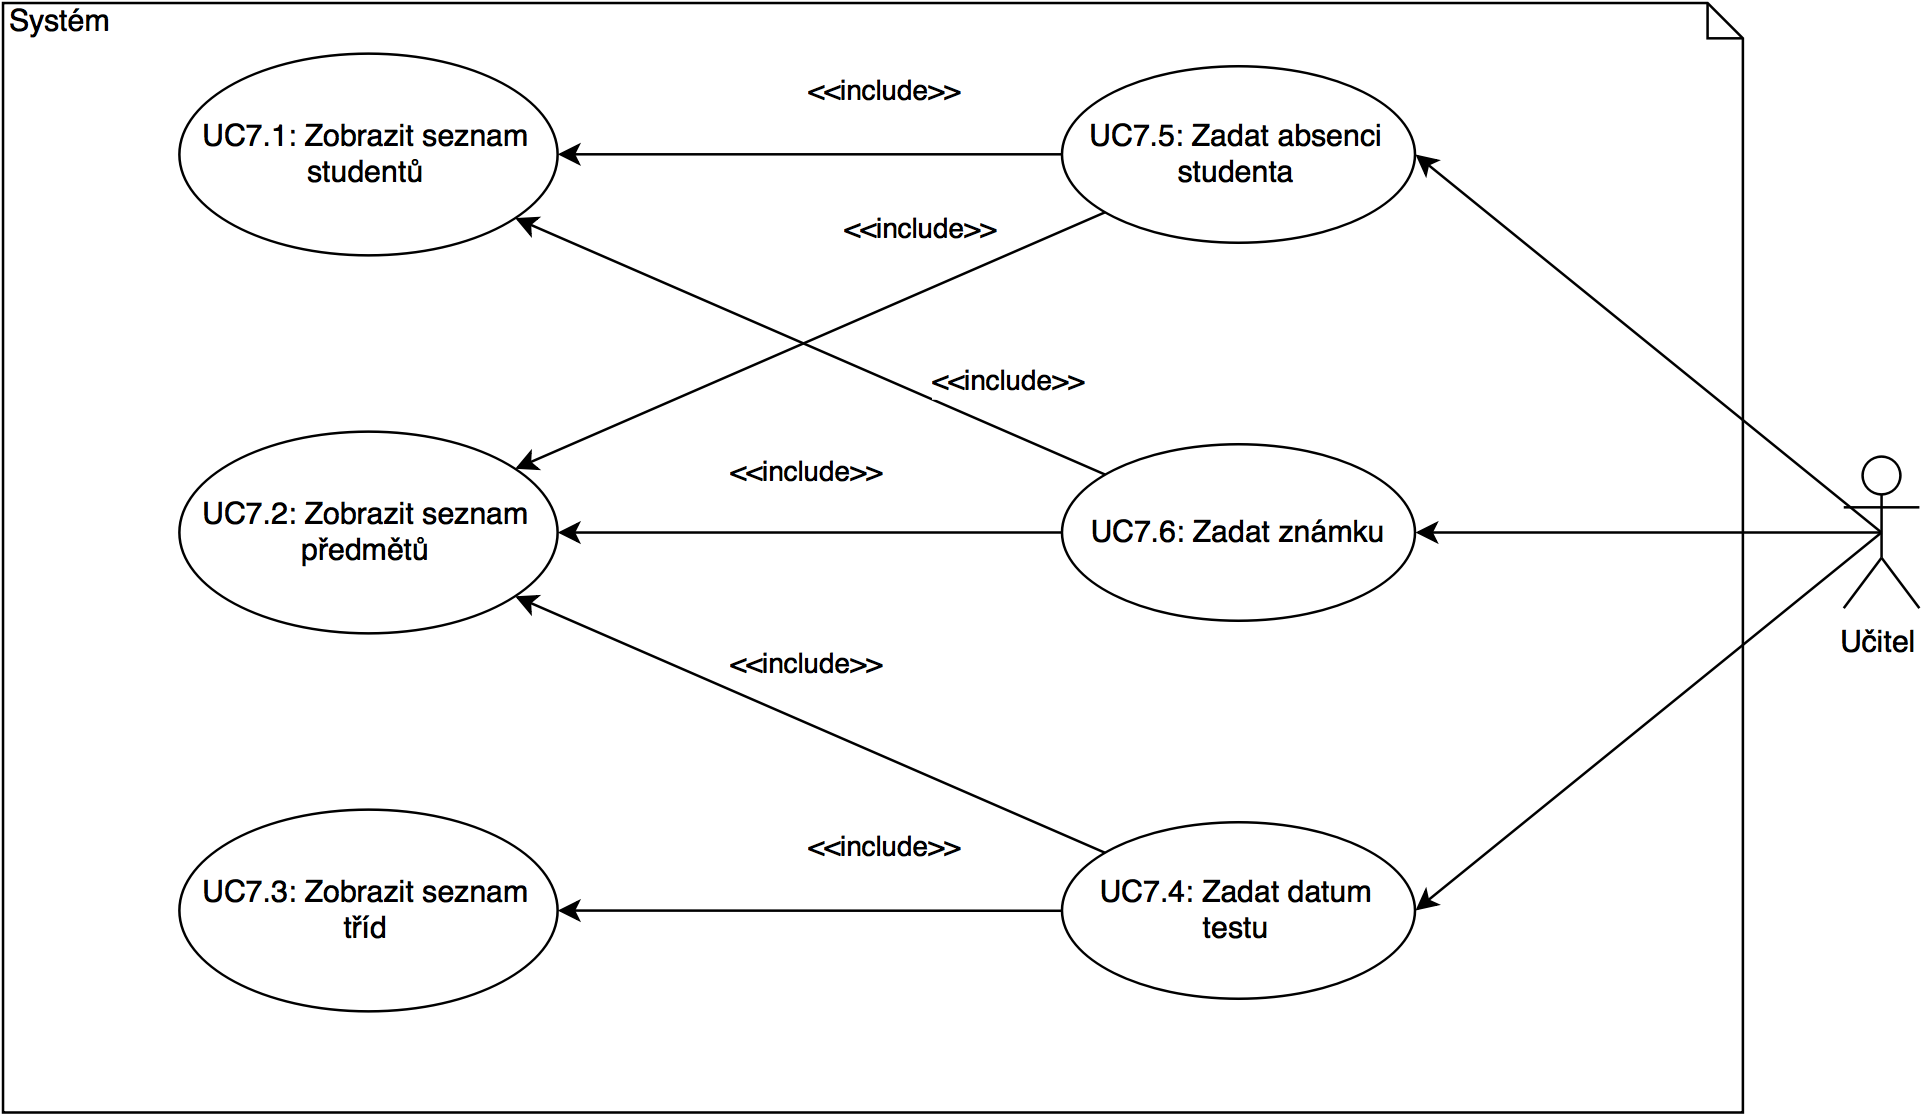
\includegraphics[width=\textwidth]{vis_use_case_diagram_7}
			\caption{UC 7 (1. úroveň)}
		\end{figure}
		\begin{figure}[h!]
			\centering
					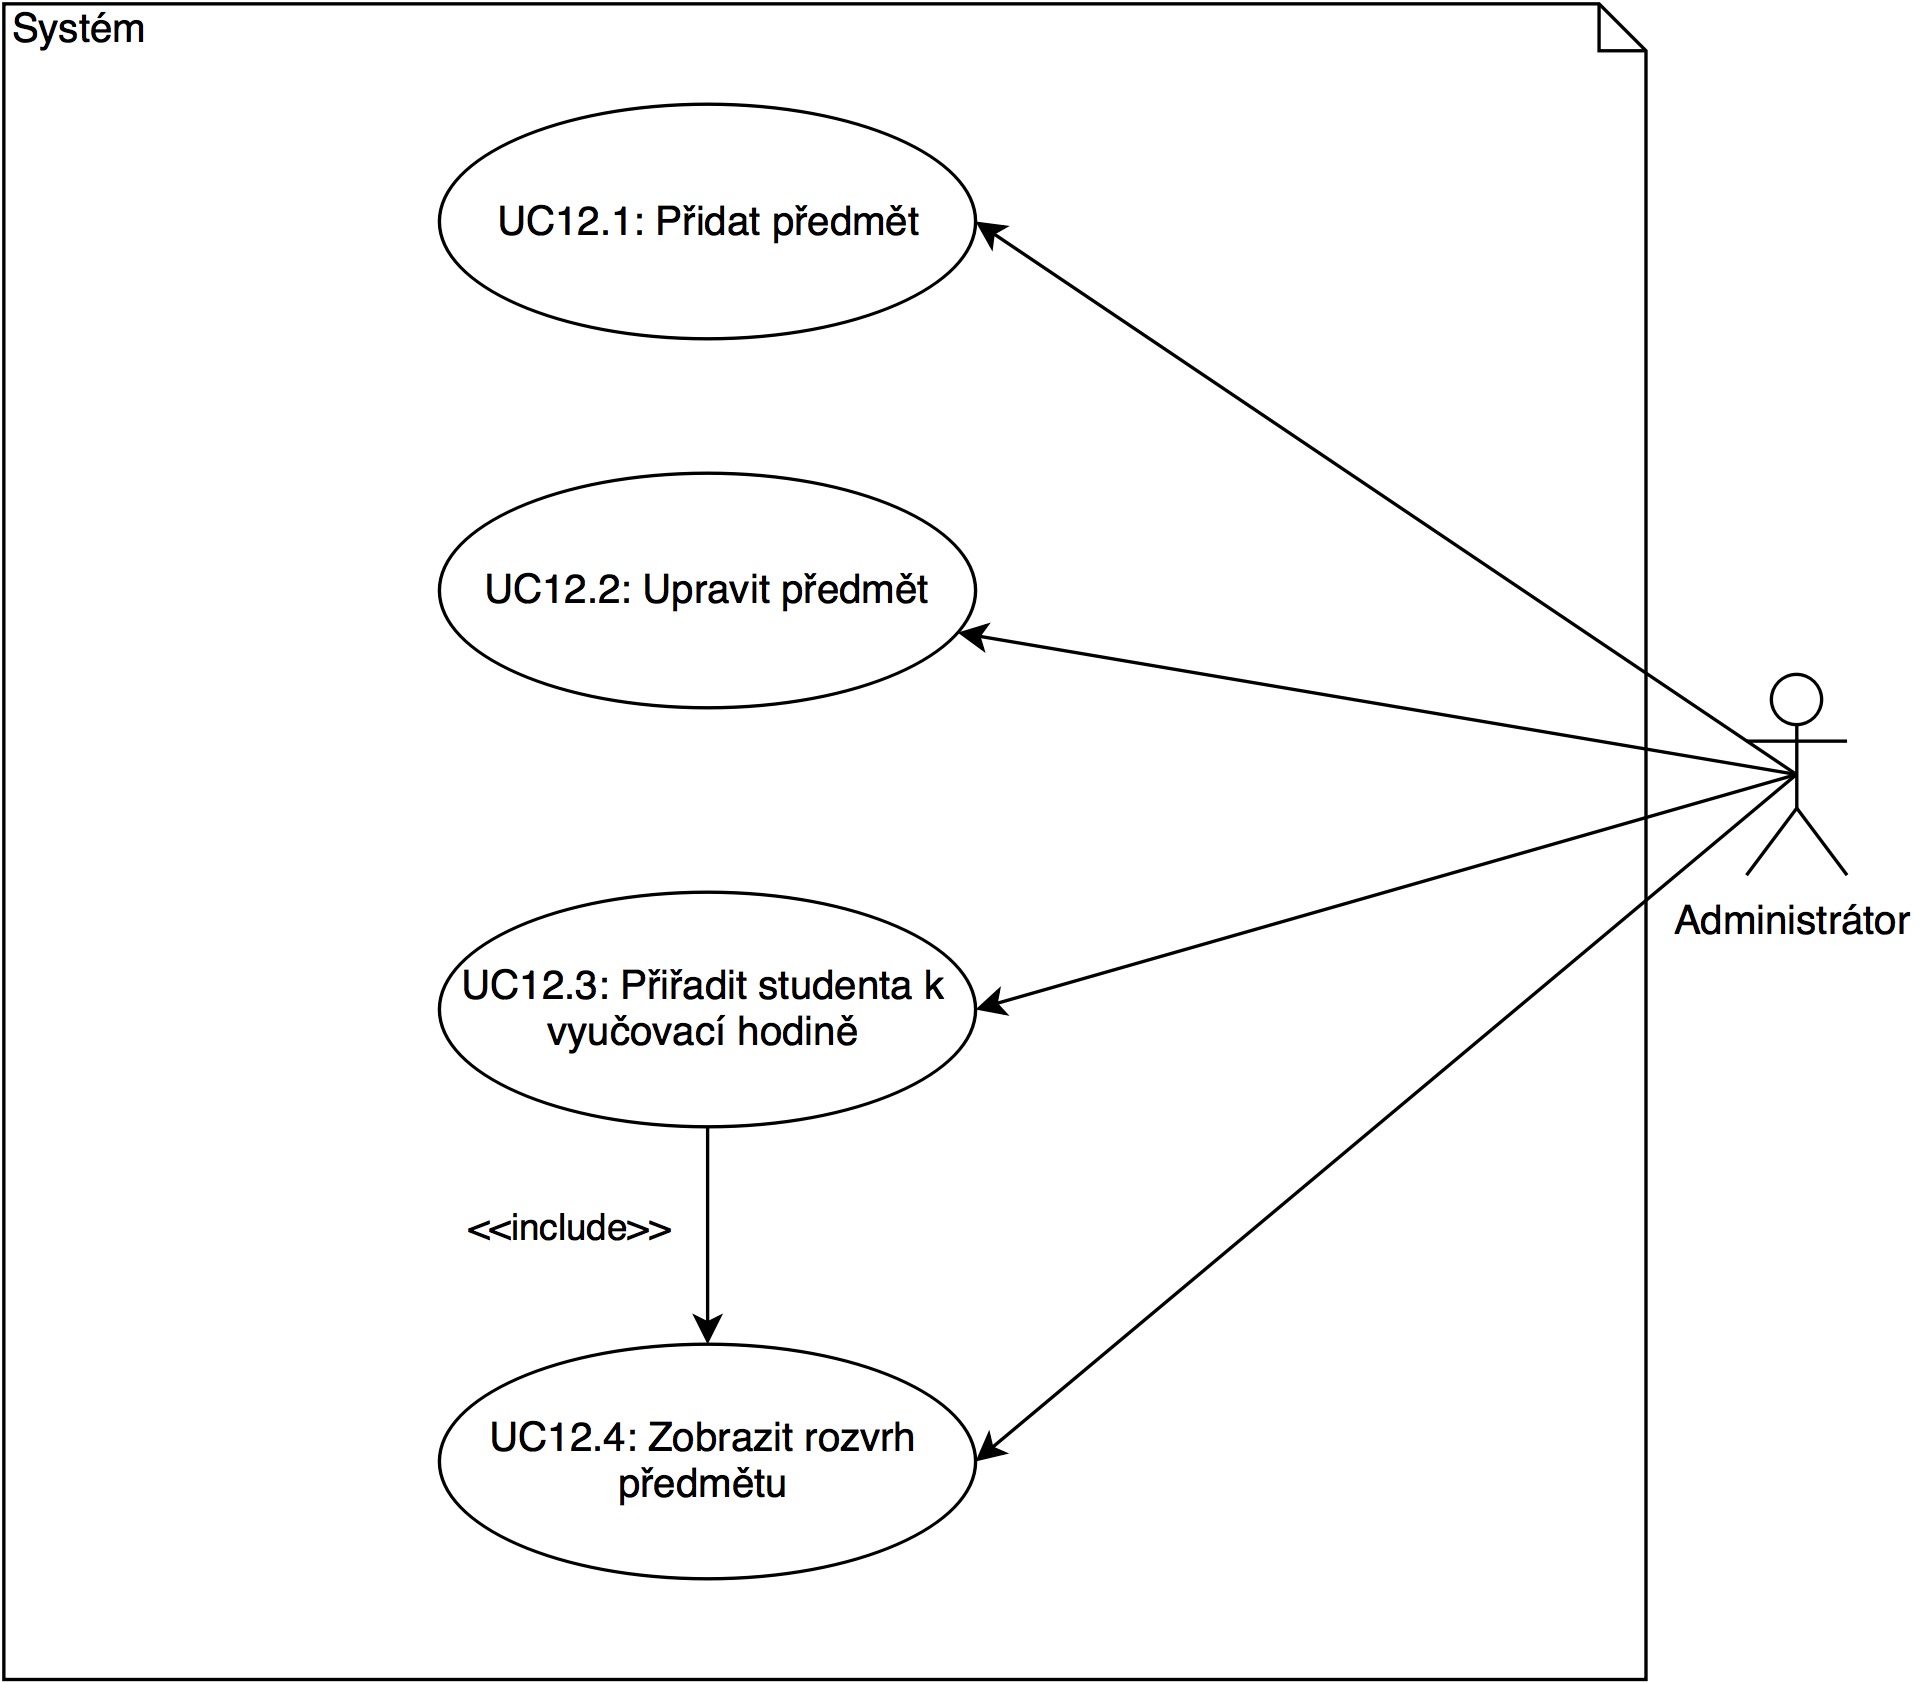
\includegraphics[width=\textwidth]{vis_use_case_diagram_12}
			\caption{UC 12 (1. úroveň)}
		\end{figure}
		
	\subsection{Případy použití}
	\subsubsection*{UC0: Přihlásit se do systému}
	\begin{description}
		\item[Popis:] Uživatel se přihlásí do systému
		\item[Aktéři:] Uživatel, systém
		\item[Prekondice:] Uživatel není přihlášený
		\item[Scénář:] \hfill
				\begin{enumerate}
					\item Systém uživatelovi zobrazí přihlašovací dialog
					\item Uživatel vyplní přihlašovací jméno, heslo a údaj, jestli má být jeho přihlášení zapamatováno
					\item Uživatel odešle údaje
					\item Systém zvaliduje zadané údaje
					\item Systém zkontroluje existenci uživatele a platnost jeho hesla
					\item Systém si zapamatuje přihlášení uživatele
					\item Systém uživatelovi zobrazí úvodní dialog systému
				\end{enumerate}
		\item[Alternativní scénář:] \hfill
				\begin{enumerate}
					\setcounter{enumi}{4}
					\setcounter{enumii}{0}
					\item \begin{enumerate}[label*=\arabic*.,leftmargin=8pt]
						\item
						\begin{enumerate}[label=\alph*.]
							\item Zadané údaje neprošly validací
							\item Systém zobrazí upozornění uživatelovi a vrátí se k bodu 2
						\end{enumerate}
						\setcounter{enumi}{5}
						\setcounter{enumii}{0}
						\item
						\begin{enumerate}[label=\alph*.]
							\item Uživatel neexistuje nebo heslo není platné
							\item Systém zobrazí upozornění uživatelovi a vrátí se k bodu 2
						\end{enumerate}
						\setcounter{enumi}{6}
						\setcounter{enumii}{0}
						\item
						\begin{enumerate}[label=\alph*.]
							\item Uživatel nesouhlasil se zapamatováním přihlášení
							\item Systém jde rovnou k bodu 7
						\end{enumerate}
					\end{enumerate}		
				\end{enumerate}
	\end{description}
	\subsubsection*{Aktivitní diagram}
		\begin{figure}[h!]
			\centering
					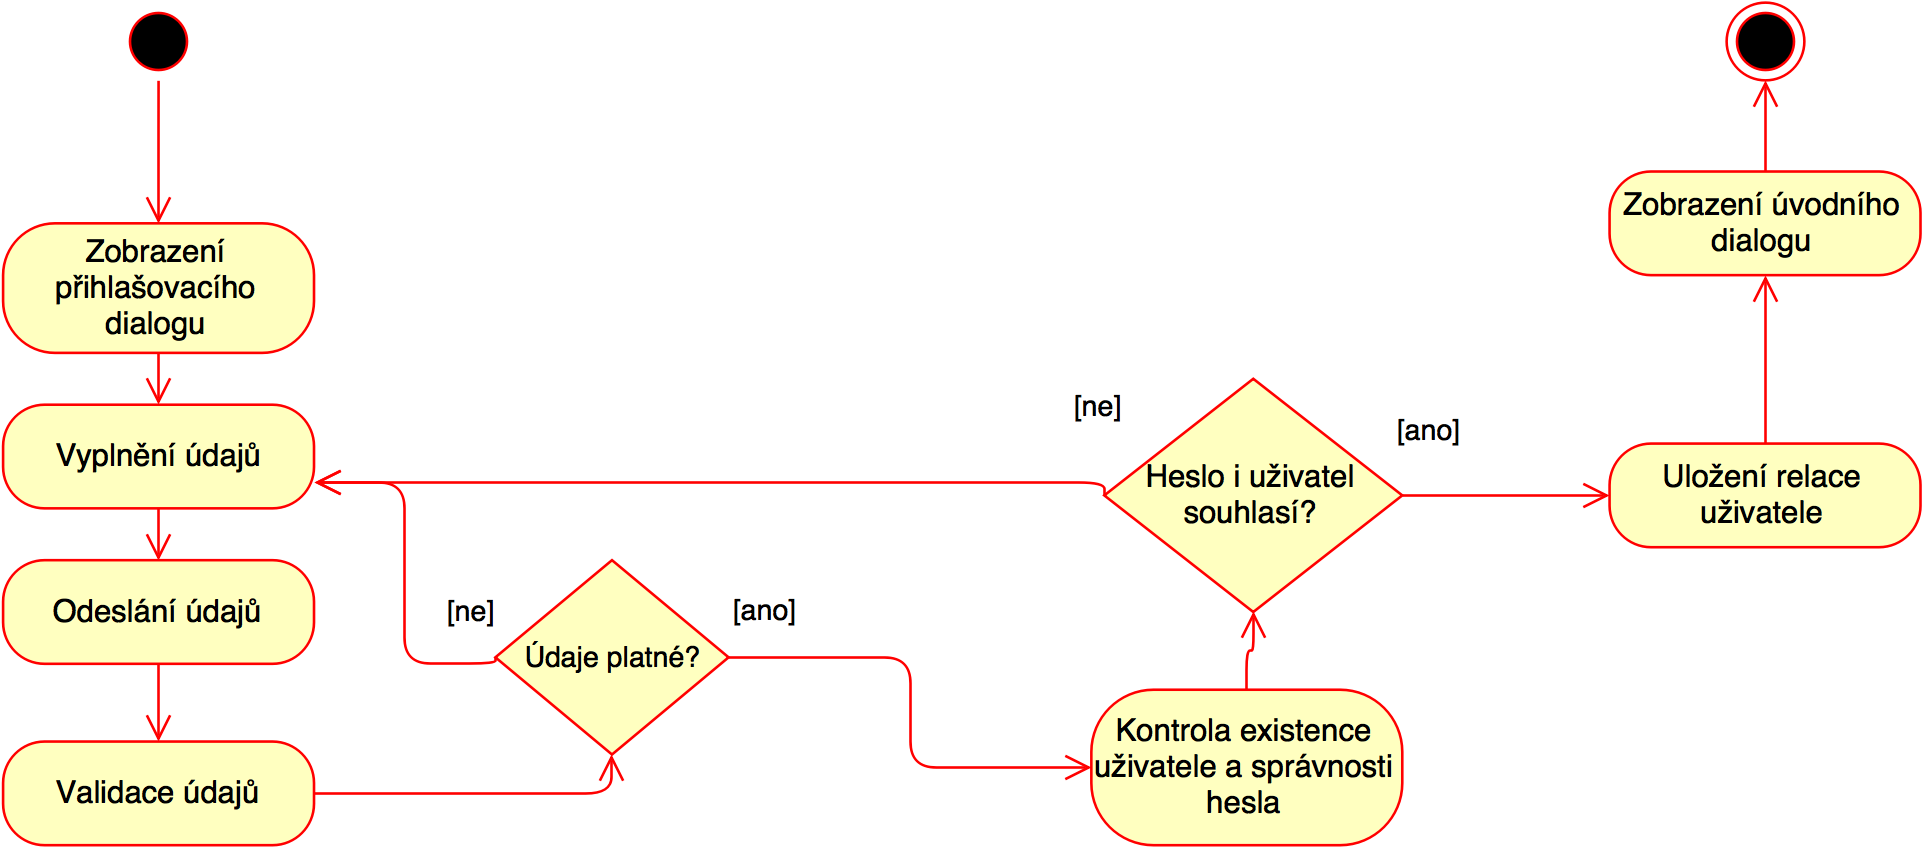
\includegraphics[width=\textwidth]{vis_uc0_activity}
			\caption{Aktivitní diagram pro UC0}
		\end{figure}
	\vspace{5mm}
	
	\subsubsection*{UC2: Přidat známky nanečisto}
	\begin{description}
		\item[Popis:] Student vytvoří známku nanečisto a systém vypočte jeho hypotetický průměr s touto známkou
		\item[Aktéři:] Student, systém
		\item[Prekondice:] Student je přihlášený
		\item[Scénář:] \hfill
				\begin{enumerate}
					\item Systém studentovi zobrazí seznam jeho známek (viz UC1)
					\item Student zvolí předmět, ke kterému chce přidat známku
					\item Student vyplní hodnotu a váhu známky
					\item Student potvrdí vytvoření známky
					\item Systém zvaliduje zadanou známku
					\item Systém vypočte nový průměr známek studenta
					\item Systém zobrazí nový průměr studentovi
				\end{enumerate}
		\item[Alternativní scénář:] \hfill
				\begin{enumerate}
					\setcounter{enumi}{5}
					\setcounter{enumii}{1}
					\item \begin{enumerate}[label*=\arabic*.,leftmargin=8pt]
						\item
							\begin{enumerate}[label=\alph*.]
								\item Známka zadaná studentem nemá platnou hodnotu
								\item Systém zobrazí upozornění studentovi a vrátí se k bodu 3
							\end{enumerate}
					\end{enumerate}		
				\end{enumerate}
	\end{description}
	\subsubsection*{Aktivitní diagram}
		\begin{figure}[H]
			\centering
					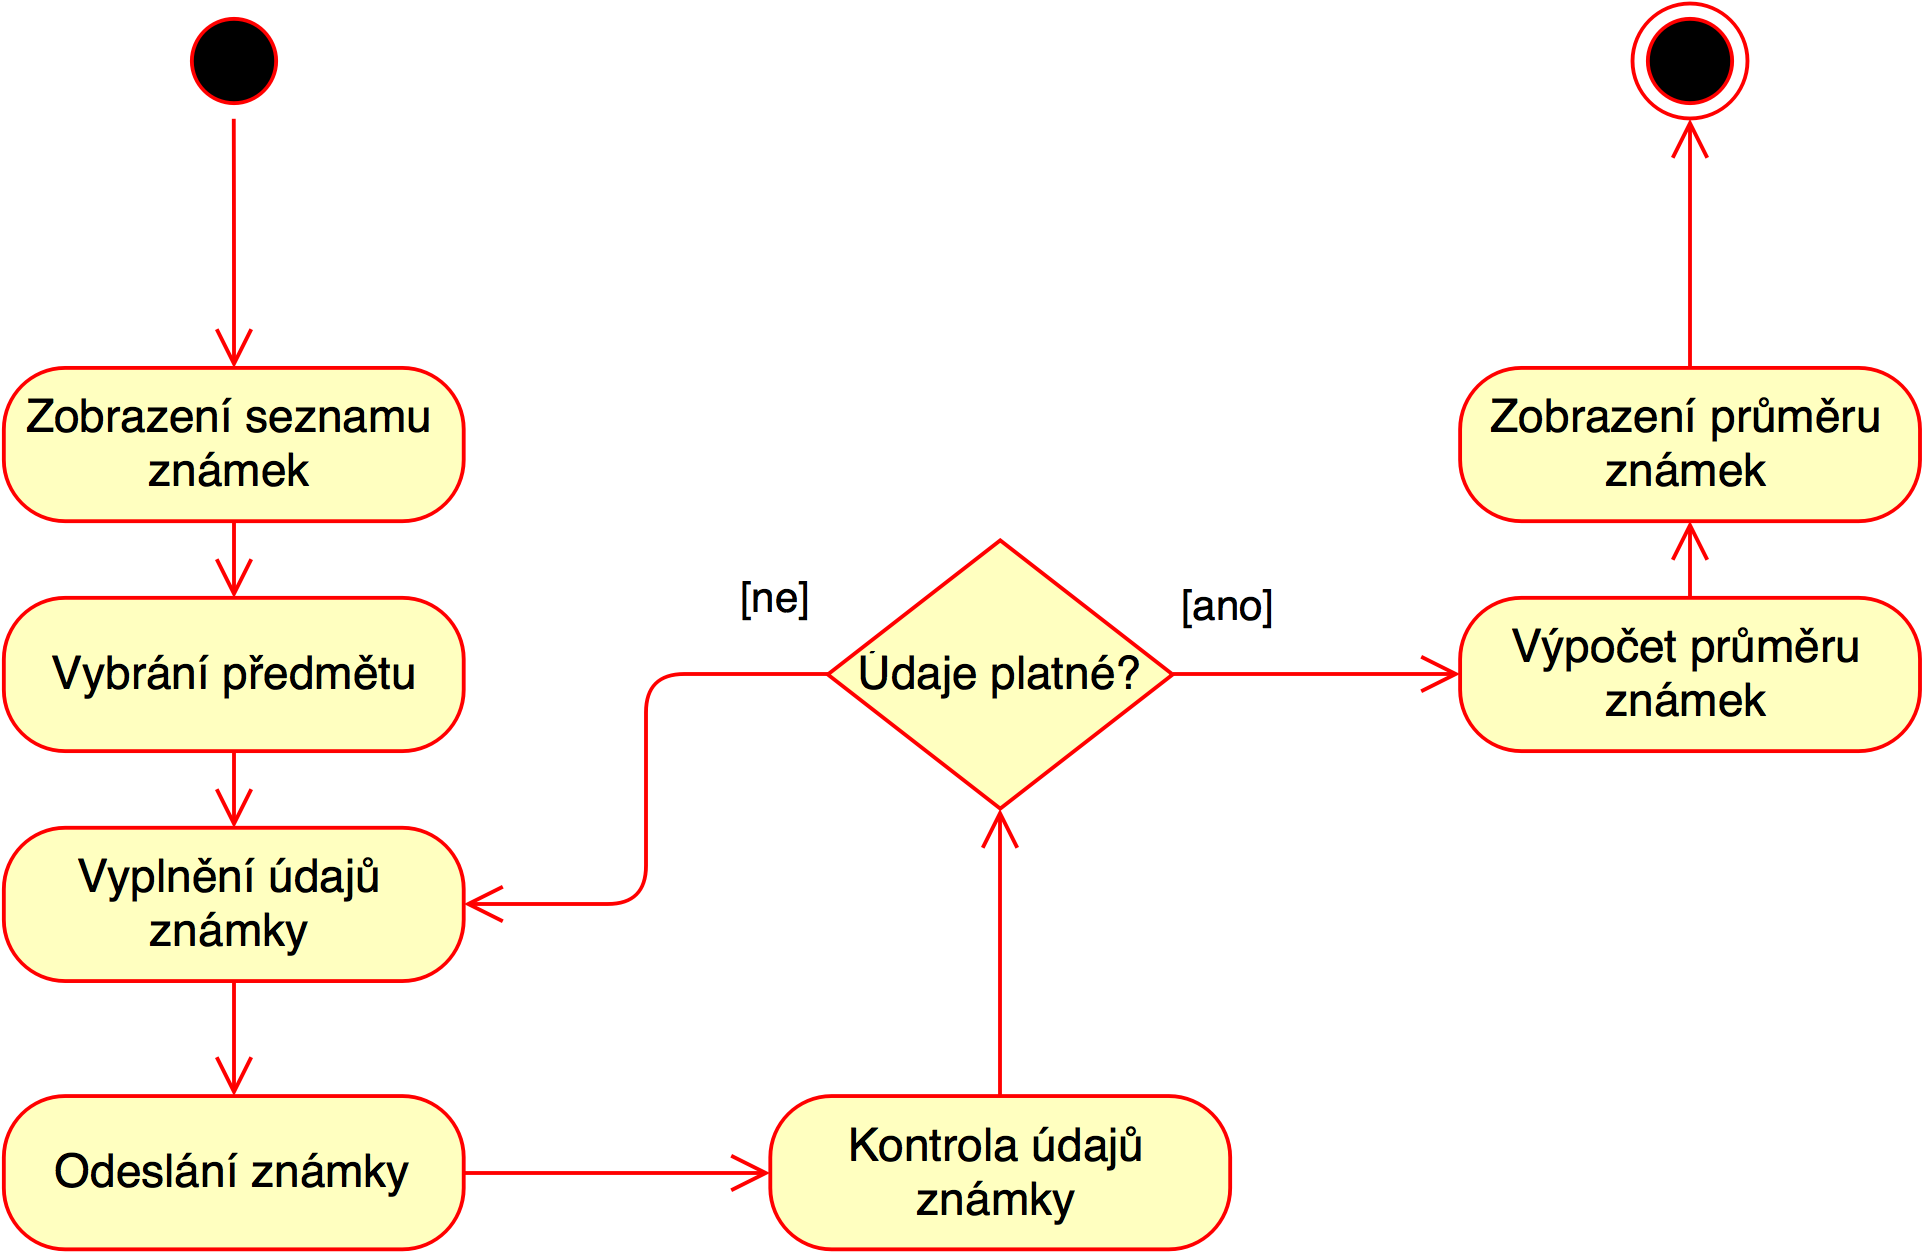
\includegraphics[width=\textwidth]{vis_uc2_activity}
			\caption{Aktivitní diagram pro UC2}
		\end{figure}
	\vspace{5mm}
	
	\subsubsection*{UC9: Přidat suplování}
	\begin{description}
		\item[Popis:] Učitel přidá do rozvrhu informaci o tom, že nebude danou vyučovací hodinu vyučovat
		\item[Aktéři:] Učitel, systém
		\item[Prekondice:] Učitel je přihlášený
		\item[Scénář:] \hfill
				\begin{enumerate}
					\item Systém učitelovi zobrazí jeho rozvrh (viz UC8)
					\item Učitel zvolí vyučovací hodinu, pro kterou chce zadat suplování
					\item Učitel odešle údaje
					\item Systém uživatelovi zobrazí seznam učitelů, kteří v danou dobu nevyučují a můžou ho suplovat
					\item Učitel zvolí učitele, který ho bude suplovat
					\item Systém uloží údaje
					\item Systém odešle e-mail zvolenému učiteli, aby o daném suplování věděl
				\end{enumerate}
		\item[Alternativní scénář:] \hfill
				\begin{enumerate}
					\setcounter{enumi}{4}
					\setcounter{enumii}{1}
					\item \begin{enumerate}[label*=\arabic*.,leftmargin=8pt]
						\item
							\begin{enumerate}[label=\alph*.]
								\item Žádný jiný učitel v danou dobu není dostupný nebo učitel zvolí, že chce nechat hodinu odpadnout
								\item Systém nastaví, že daná hodina odpadne
								\item Systém odešle e-mail studentům dané hodiny, že tato hodina odpadá
								\item Scénář užití končí
							\end{enumerate}
					\end{enumerate}		
				\end{enumerate}
	\end{description}
	\subsubsection*{Aktivitní diagram}
		\begin{figure}[H]
			\centering
					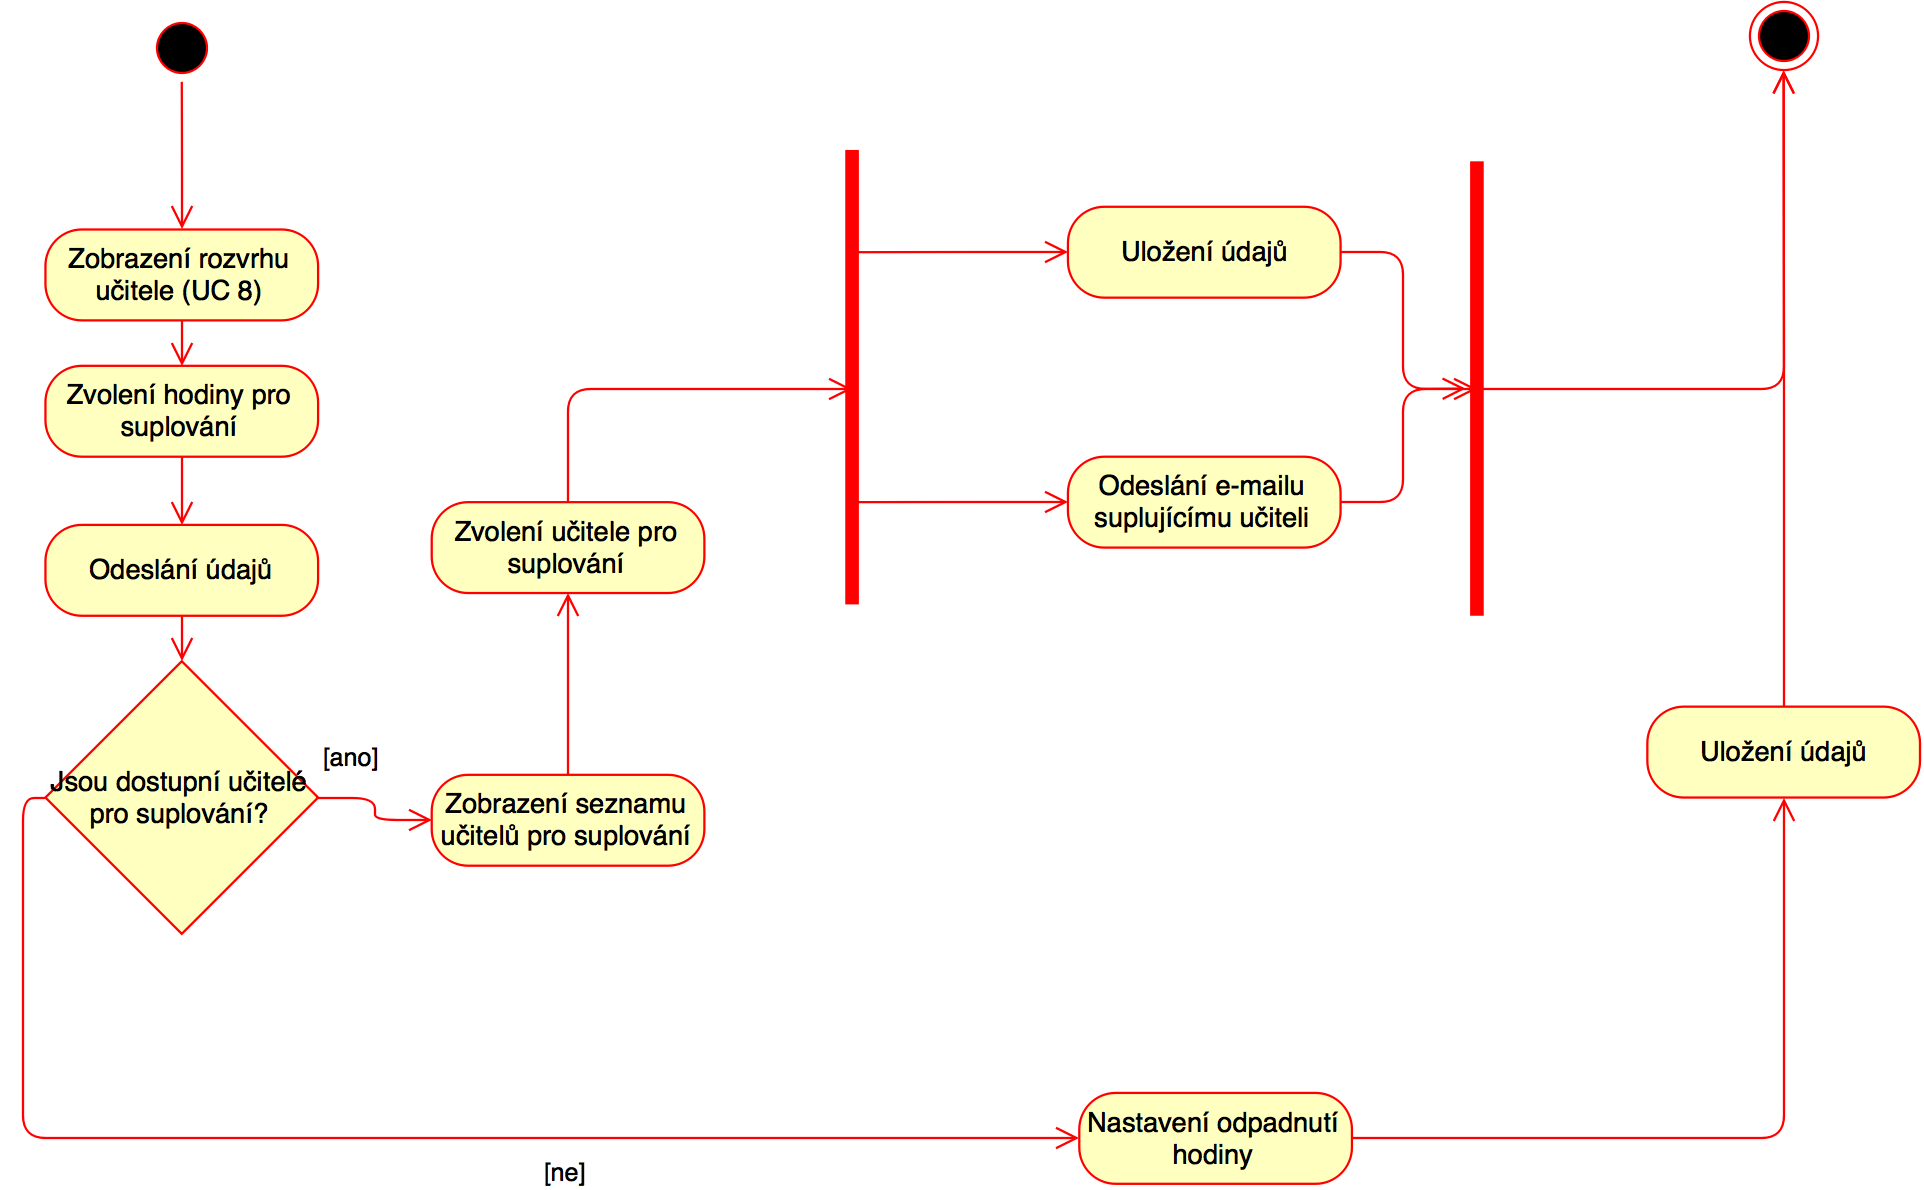
\includegraphics[width=\textwidth]{vis_uc9_activity}
			\caption{Aktivitní diagram pro UC9}
		\end{figure}
	\vspace{5mm}
	
	\section{Technická specifikace}
	\subsection{Konceptuální model domény}
		\begin{figure}[H]
			\centering
					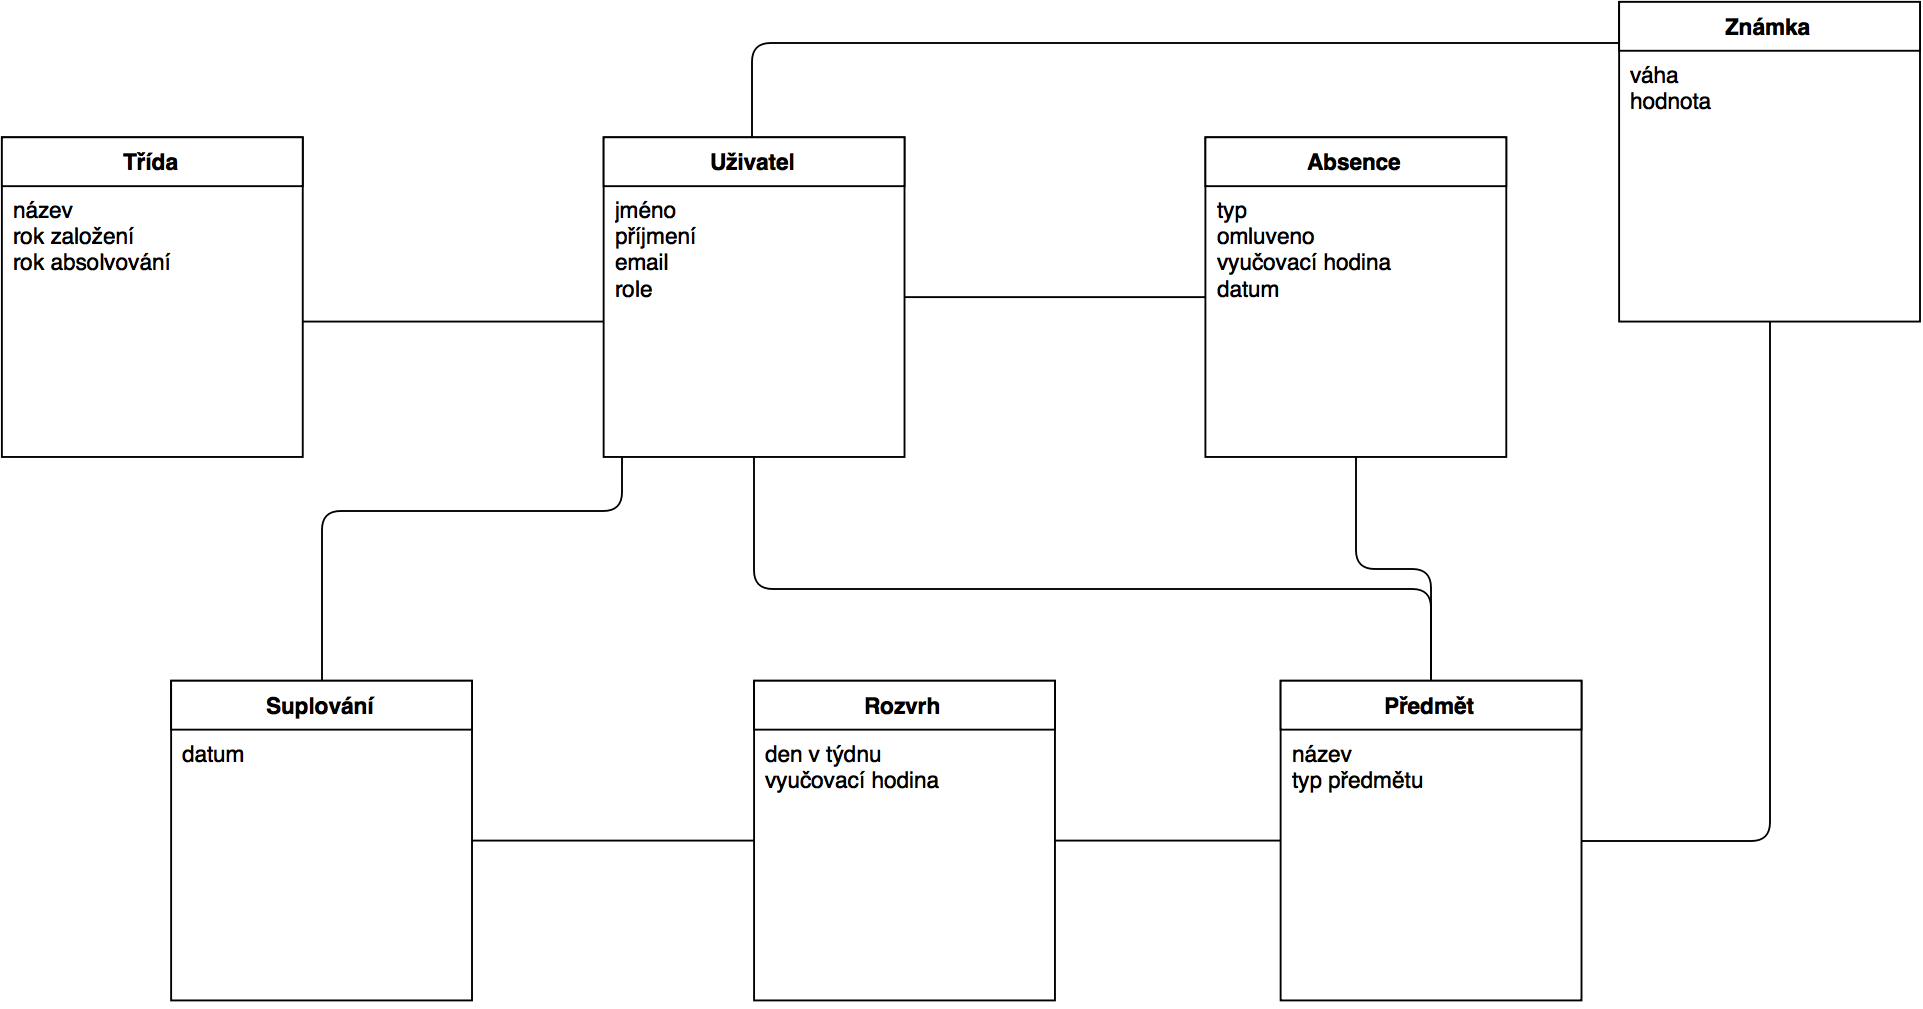
\includegraphics[width=\textwidth]{vis_conceptual_domain_model}
			\caption{Konceptuální model domény}
		\end{figure}
			
	\subsection{Technologie}
		Systém bude vytvořen v jazyce C\# a frameworku .NET. Tato technologie byla vybrána, protože se jedná o moderní technologii, která je aktivně vyvíjena a podporována firmou Microsoft, obsahuje velkou spoustu zdarma dostupných knihoven, které značne urychlují vývoj programů, a aplikace je v ní možné vyvíjet pomocí vývojových prostředí dostupných zdarma. Jako databáze bude použit Microsoft SQL Server, jelikož má dobrou
		kompatibilitu s platformou .NET. Systém nebude muset ukládat velké objemy dat, postačí tedy verze SQL Server Express, která je dostupná zdarma.
		Z důvodu rozložení zátěže a většího zabezpečení bude systém rozdělen na dva počítače - databázový server, starající se o
		úschovu dat, který nebude připojený k internetu, a aplikační server, který bude poskytovat rozhraní k systému přes internet a bude také obsahovat
		samotnou aplikační logiku systému. K aplikačnímu serveru se budou klienti připojovat přes internet buď z webového prohlížeče nebo z mobilního zařízení
		se systémem Android. Tento server bude komunikovat s databázovým serverem po místní síti. Veškerá komunikace se systémem bude probíhat po internetu, takže
		aplikační server bude muset mít dostatečnou kapacitu připojení k internetu. K systému bude připojených naráz maximálně 50-100 uživatelů, velikost jedné
		načtené stránky bude cca. 500 KiB. Při tomto počtu uživatelů můžeme počítat zhruba s dvěmi načteními stránky za vteřinu, kapacita internetové linky
		serverů by měla tedy být alespoň 10 Mbit/s.
		\begin{enumerate}
			\item Aplikační server
				\begin{description}
					\item[Popis:] \hfill \\Tento server bude obsahovat aplikační logiku systému skrytou za webovou službou, ke které budou moci klienti přistupovat přes
						internet z mobilní aplikace. Dále bude obsahovat webový server, ke kterému budou uživatelé přistupovat pomocí prohlížeče.
						Jelikož systém bude běžet pod prostředím .NET, operační systém tohoto serveru bude Microsoft Windows Server, pro zajištění maximální kompatibility
						a jednoduchosti vývoje. Tento server bude kombinovat webový server i aplikační logiku, bude tedy potřebovat alespoň 8 GiB RAM paměti.
						Protože server bude běžet neustále, bude ideální pro něj použít procesor Intel Xeon, který je navržen pro neustálý běh a nízkou energetickou spotřebu.
						Na tomto serveru se nebudou uchovávat data systému, postačí pro něj tedy základní pevný disk o kapacitě 250 GiB.
					\item[Operační systém:] Microsoft Windows Server 2012
					\item[Software:] .NET framework ve verzi 4.5
					\item[Hardware:] Intel Xeon E3-1220 (3.1 GHz), 8 GiB RAM, WD Blue HDD 250 GiB
				\end{description}
			\item Databázový server
			\begin{description}
				\item[Popis:] \hfill \\Tento server bude obsahovat databázi informačního systému, ke které bude aplikační server přistupovat přes místní síť.
						Jelikož dat v databázi nebude hodně (viz odhad dat níže), postačí serveru 4 GiB operační paměti. Do operační paměti by se měla vlézt celá databáze, takže nebude potřeba použít SSD disky, které jsou sice rychlejší, ale dražší. Tento server tedy bude mít dva pevné disky, zapojené v módu RAID 1 (zrcadlení) pro možnost obnovení dat při potenciální závadě disku.  Stejně jako aplikační server bude běžet neustále, použije se pro něj tedy procesor Intel Xeon.
				\item[Operační systém:] Microsoft Windows Server 2012
				\item[Software:] .NET framework ve verzi 4.5, Microsoft SQL Server Express
				\item[Hardware:] Intel Xeon E3-1220 (3.1 GHz), 4 GiB RAM, 2x WD RE Raid Edition HDD 250 GiB
			\end{description}
		\item Klient (prohlížeč)
			\begin{description}
				\item[Popis:] \hfill \\Uživatelé budou moci přistupovat k systému pomocí standardního webového prohlížeče.
				\item[Operační systém:] Libovolný
				\item[Software:] Nové verze nejvíce používaných prohlížečů (Opera, Google Chrome, Mozilla Firefox, Microsoft Internet Explorer aj.)
			\end{description}
		\item Klient (mobilní zařízení)
			\begin{description}
				\item[Popis:] \hfill \\Uživatelé budou moci přistupovat k systému pomocí nativní aplikace pro systém Android.
				\item[Operační systém:] Android OS 2.3+
			\end{description}
		\end{enumerate}
	\subsection{Odhad objemu dat}
		Tato tabulka znázorňuje odhad velikosti dat uložených v systému po jednom roce aktivního používání.
		\\\\
		\begin{tabular}{| c | c | c | c |}
			\hline
			Entita & Velikost [B] & Počet & Celková velikost [KiB] \\ \hline
			Uživatel & 100 & 800 & 80 \\ \hline
			Třída & 80 & 20 & 1,6 \\ \hline
			Suplování & 20 & 200 & 4 \\ \hline
			Rozvrh & 30 & 500 & 15 \\ \hline
			Absence & 30 & 500 & 15 \\ \hline
			Předmět & 30 & 50 & 1,5 \\ \hline
			Známka & 20 & 50000 & 1000 \\
			\hline
		\end{tabular}
		
		\section{Skica uživatelského rozhraní}
			\begin{figure}[H]
				\centering
					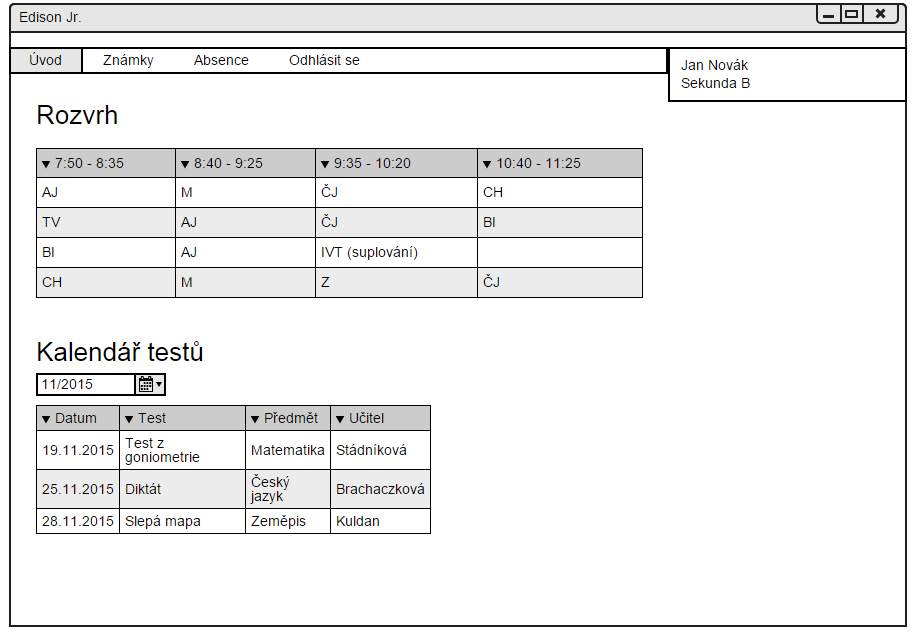
\includegraphics[width=\textwidth]{vis_wireframe_student}
				\caption{Student: rozvrh hodin a kalendář testů}
			\end{figure}
			\begin{figure}[H]
				\centering
						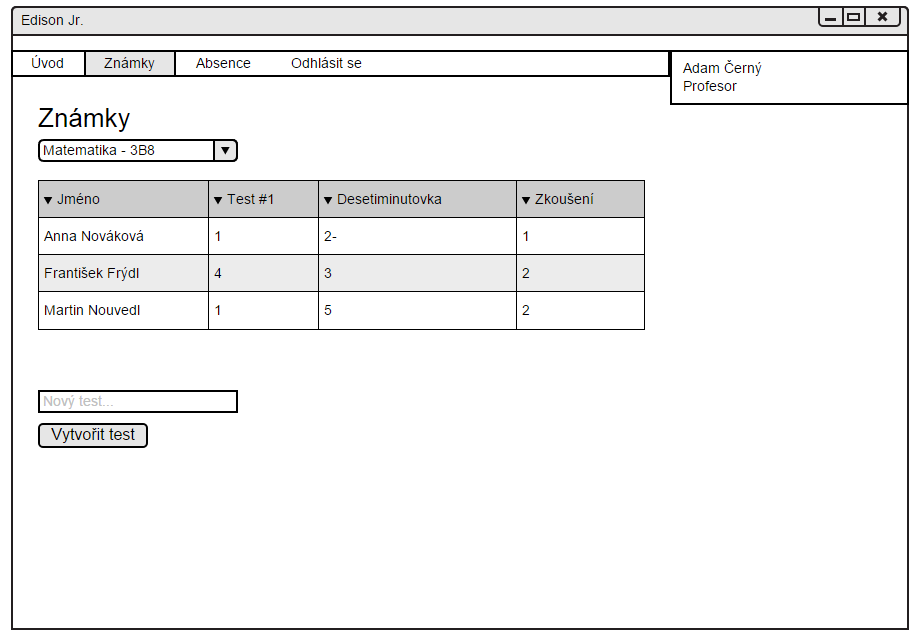
\includegraphics[width=\textwidth]{vis_wireframe_ucitel}
				\caption{Učitel: zadávání známek a vytváření testů}
			\end{figure}
		\section{Návrh doménového modelu}
			\subsection{Aplikace návrhových vzorů}
				\subsubsection*{Prezentační vrstva}
					Prezentační vrstva bude získávat data ze servisní vrstvy. Pro přístup k ní bude využívat bránu (\textbf{Gateway}), aby
					nemusela přímo znát implementační detaily používání služby a servisní vrstva pro ni byla transparentní.
					Data ze servisní vrstvy budou navrácena v podobě datových obálek (\textbf{Data Transfer Object}).
					Webová aplikace bude založená na modelu MVC (\textbf{Model-View-Controller}), aby se důsledně oddělila prezentace dat a logika aplikace.
					Controllery budou mít jednoho společného předka (\textbf{Front controller}), který se bude starat o logiku společnou pro všechny stránky na
					webu, jako je nastavování jazyku, načítání relace nebo obsluha chyb. Dále pak bude obsahovat samostatné controllery pro každou část webu
					(\textbf{Page controller}). Relace uživatelů bude běžet na samotném webovém serveru (\textbf{Server session state}). Pro vykreslování
					HTML budou použity šablonované pohledy (\textbf{Template view}). Pro prezentační vrstvu na mobilních zařízeních bude použit
					\textbf{MVC} a \textbf{Gateway}.
			
				\subsubsection*{Servisní vrstva}
					Servisní vrstva bude poskytovat rozhraní k přístupu k doménové logice pro prezentační vrstvu.
					Pro přenos objektů budou použity jednoduché datové obálky (\textbf{Data Transfer Object}), aby se zjednodušila serializace
					objektů pro přenos po síti a aby klienti služby neměli závislost na fyzické komponentě (DLL souboru) doménové vrstvy.
					Jednotlivé metody servisní vrstvy budou vyřizovat vždy jeden požadavek od prezentační vrstvy, bude se tedy jednat o \textbf{Transakční skript}.
			
				\subsubsection*{Doménová vrstva}
					Pro modelování logiky a vztahů v doménové vrstvě bude použit \textbf{Doménový model}. Tímto se zajistí co nejvěrnější modelování reality, oddělení
					závislostí a také snazší rozšiřitelnost systému. Každý objekt bude dědit ze společného doménového předka (\textbf{Layer supertype}),
					který bude zajišťovat identifikaci objektů pomocí celočíselného klíče (\textbf{Identity field}) pro jejich snažší perzistenci.
					Bude zde také rozhraní repozitáře objektů, které bude sloužit k jejich vyhledávání a bude implementované datovou vrstvou (\textbf{Separated interface}).
				
				\subsubsection*{Datová vrstva}
					Pro mapování doménových objektů do perzistentního úložiště bude použit \textbf{Data mapper}. Zajistí se tak totální nezávislost
					doménové vrstvy na použité perzistentní technologii i na datové vrstvě. Mappery budou mít společného předka (\textbf{Layer supertype})
					zajišťujícího společnou funkcionalitu (např. připojení k DB u databázových mapperů, načítání XML souborů u XML mapperů atd.).
					Objekty načítané z perzistentního úložiště budou cachovány v procesu aplikace (\textbf{Identity map}), což zajistí větší rychlost jejich vyhledávání
					a také usnadní konzistenci mapování. Atributy doménových objektů, které budou moc velké pro okamžité načtení, se budou načítat až v době potřeby
					(\textbf{Lazy load}). Aby doménové 	objekty nevěděly o tom, že jejich atributy nejsou ještě načtené, bude jejich reálný typ skryt za rozhraním.
					Pro doménové objekty s vazbou agregace bude použito mapování cizího klíče (\textbf{Foreign key mapping}), pro některé objekty s vazbou
					kompozice (Předmět, Rozvrh) bude použito závislostní mapování jejich částí (\textbf{Dependent mapping)}.
					Jednoduché objekty, sloužící v podstatě jako výčtový typ (Vyučovací hodina) budou mapovány přímo do tabulek ostatních tříd (\textbf{Embedded value}).
					Pro mapování uživatelů, kteří dědí z abstraktní třídy Osoba, bude použito mapování do jedné tabulky (\textbf{Single table inheritance}),
					jelikož jednotlivé typy uživatelů se liší hlavně chováním a svou rolí, atributy jen minimálně. Navíc tak bude umožněno hledat v perzistentním úložišti
					jednotně (polymorficky) osoby podle společných atributů. Mappery budou konfigurovány při spuštění servisní vrstvy z XML souboru(\textbf{Plugin},
					\textbf{Metadata mapping}). Jejich závislosti (např. na databázi) jim budou vloženy při jejich vytvoření (\textbf{Dependency injection}).
					Přístup k mapperům bude zajištěn pomocí registru mapperů (\textbf{Registry}), který bude obsahovat mapper pro každou třídu z doménové vrstvy.
					K mapperu registrů bude statický přístup pro jednoduché vyhledávání objektů. Bude zároveň implementovat repozitář z doménové vrstvy, aby k objektům
					měly snadný přístup i doménové objekty (bez toho, aby věděly, že se vyhledávané objekty načítají z perzistentního úložiště).
		
			\subsection{Třídní diagram doménové vrstvy}
				\begin{figure}[H]
					\centering
							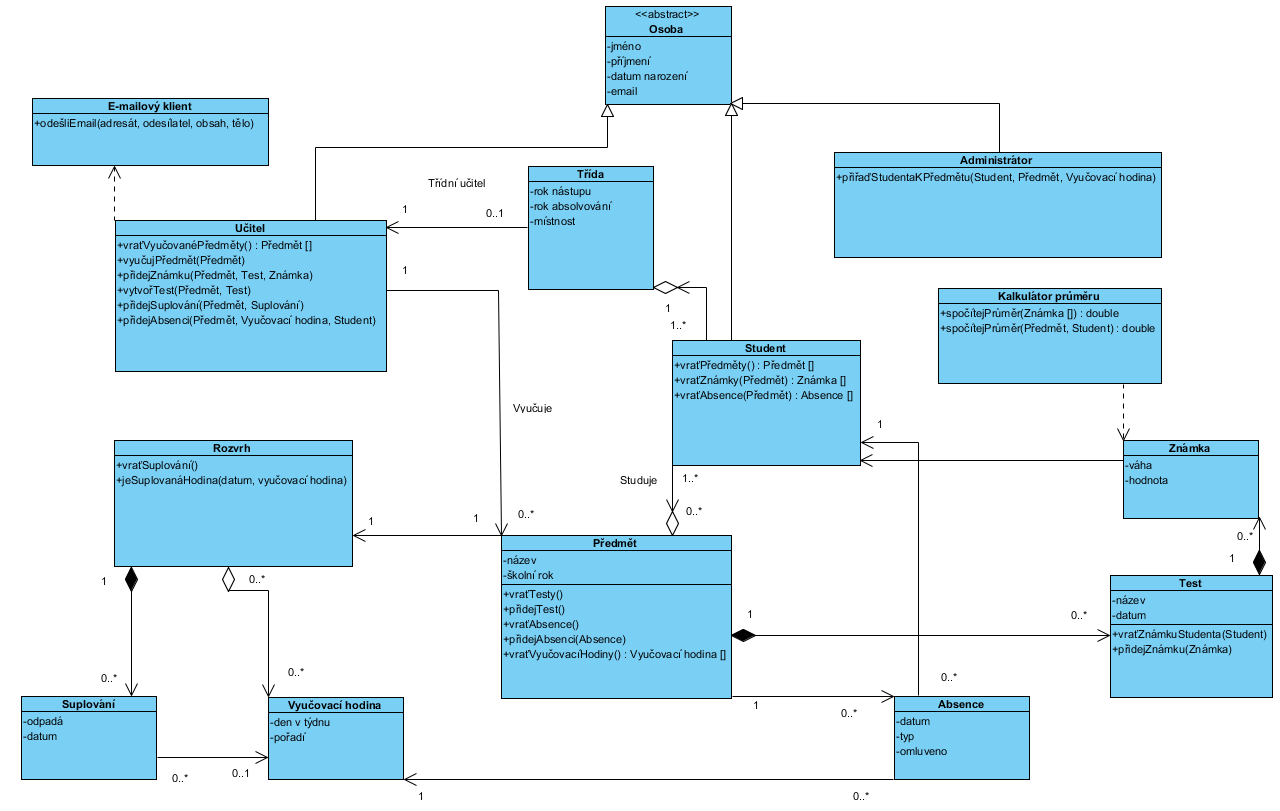
\includegraphics[width=\textwidth]{vis_class_diagram_domain}
					\caption{Doménová vrstva systému}
				\end{figure}
			\subsection{Třídní diagram datové vrstvy}
				\begin{figure}[H]
					\centering
							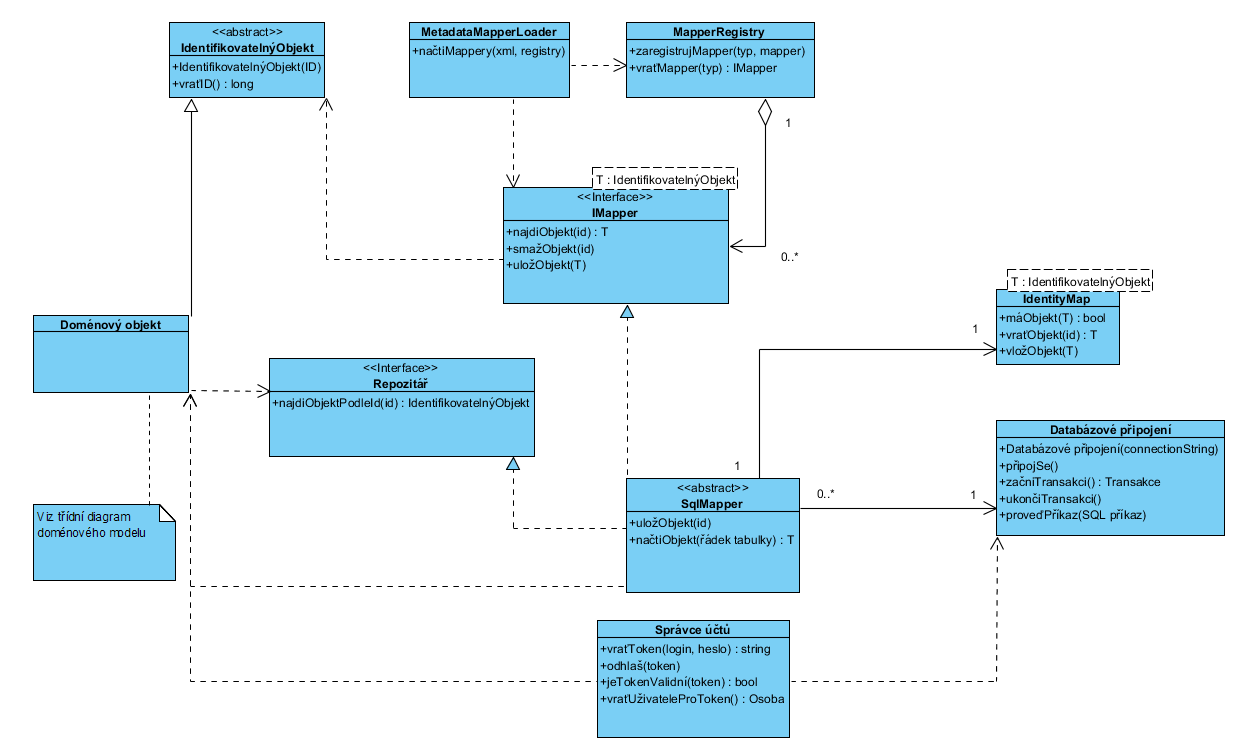
\includegraphics[width=\textwidth]{vis_class_diagram_data}
					\caption{Datová vrstva systému}
				\end{figure}
			\subsection{Sekvenční diagramy}
				\begin{figure}[H]
					\centering
							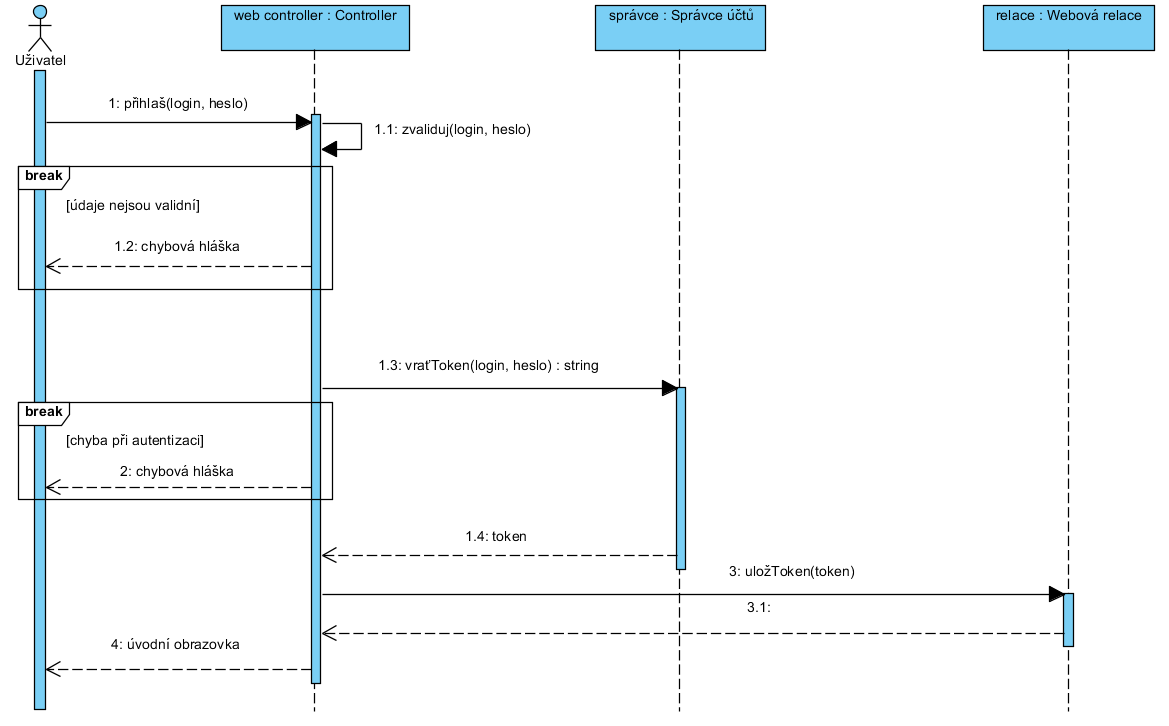
\includegraphics[width=\textwidth]{vis_sequence_diagram_uc0}
					\caption{Sekvenční diagram k UC0}
				\end{figure}
				\begin{figure}[H]
					\centering
							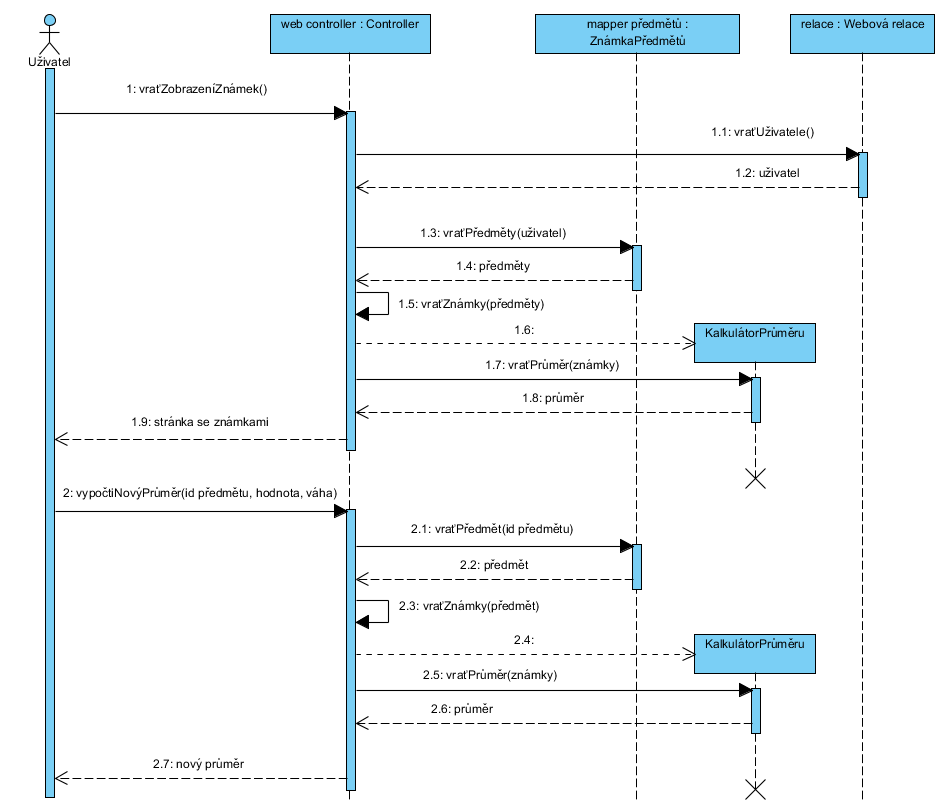
\includegraphics[width=\textwidth]{vis_sequence_diagram_uc2}
					\caption{Sekvenční diagram k UC2}
				\end{figure}
				\begin{figure}[H]
					\centering
							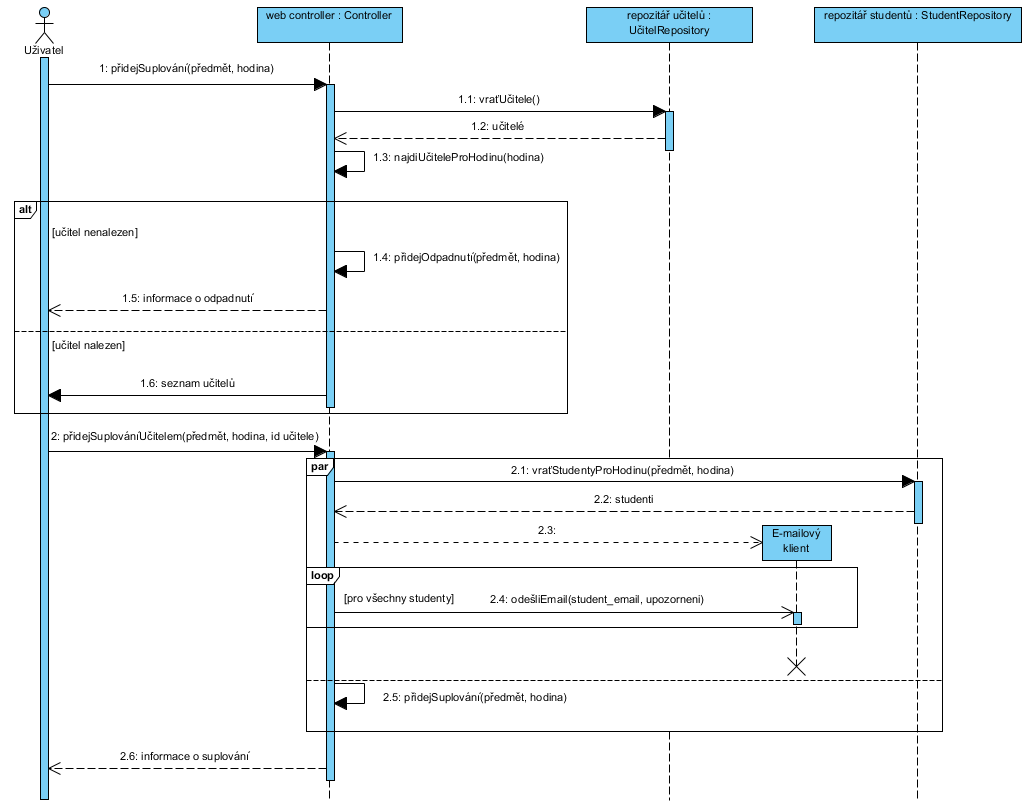
\includegraphics[width=\textwidth]{vis_sequence_diagram_uc9}
					\caption{Sekvenční diagram k UC9}
				\end{figure}
		\section{Architektura systému}
			\subsection{Komponenty systému}
					\begin{figure}[H]
						\centering
								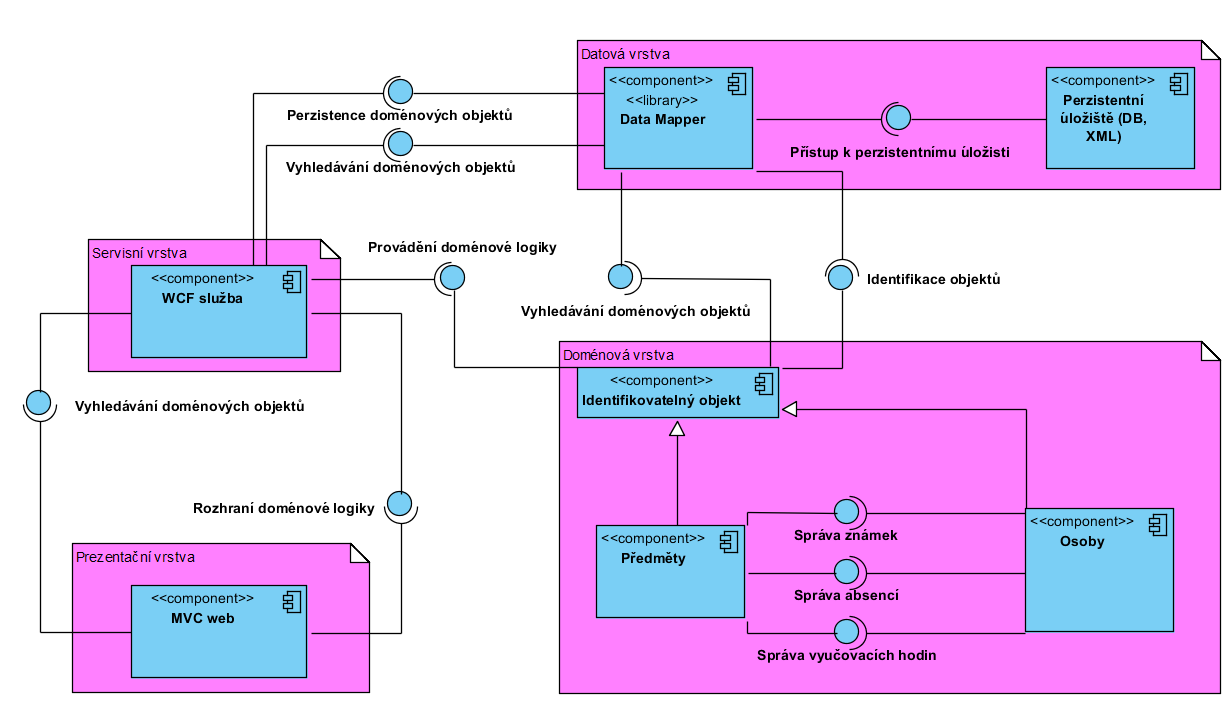
\includegraphics[width=\textwidth]{vis_component_diagram}
						\caption{Diagram komponent}
					\end{figure}
			\subsection{Rozložení fyzických a logických vrstev}
				Systém bude rozložen do třívrstvé architektury s použitím servisní vrstvy mezi prezentační a doménovou vrstvou.
				Prezentační vrstva bude jak u klienta (webový prohlížeč, mobilní aplikace), tak na aplikačním serveru (webová aplikace).
				Servisní vrstva bude běžet aplikačním serveru, společně s doménovou a datovou vrstvou.
				Databáze bude běžet odděleně na databázovém serveru.
				Uživatelé systému k němu budou přistupovat buď z webového prohlížeče anebo z mobilní aplikace.
				Na aplikačním serveru bude běžet webový server pro obsluhu prohlížečů. Ten bude využívat servisní vrstvy
				implementované pomocí technologie WCF (Windows Communication Foundation). Tato služba bude poskytovat externí rozhraní
				pro doménový model a zároveň bude možné se k ní rovnou připojit z mobilní aplikace. Jelikož tuto službu bude využívat i webové rozhraní, zabrání
				se duplicitě kódu při přístupu k doménové vrstvě.
				\begin{figure}[H]
					\centering
							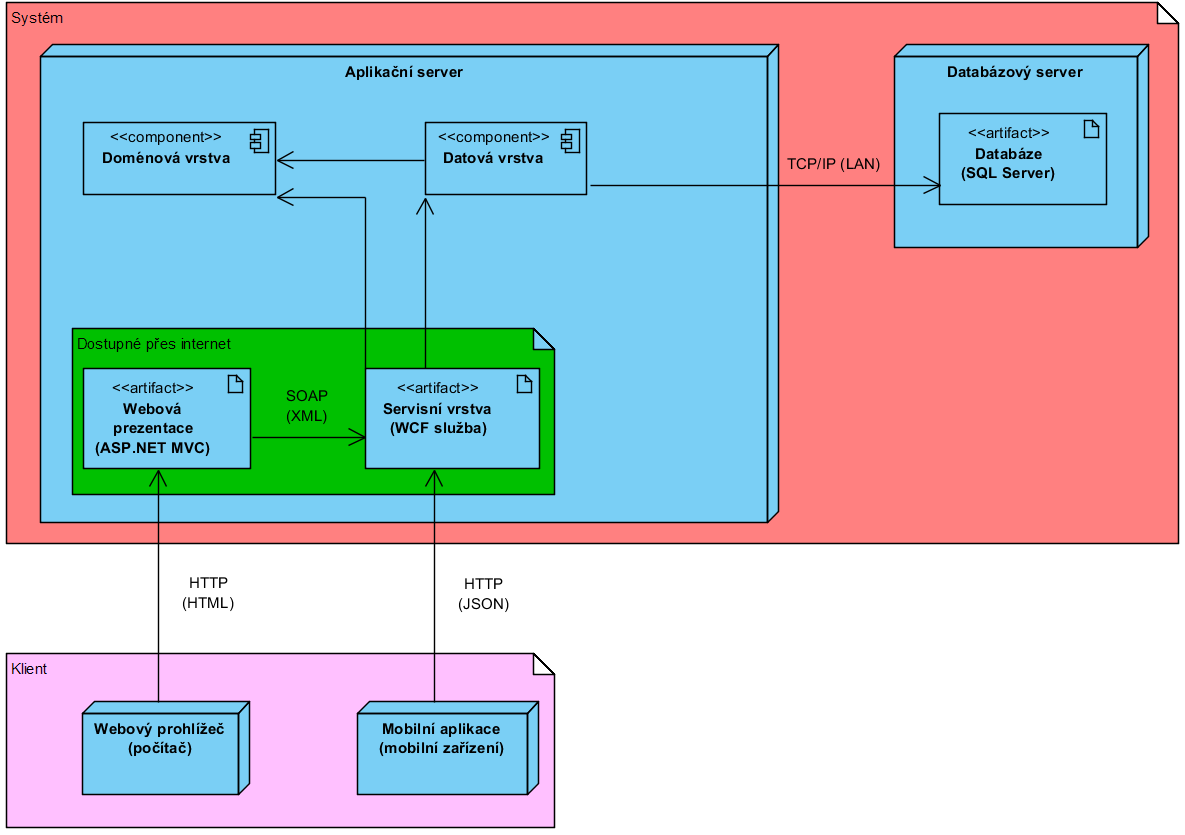
\includegraphics[width=\textwidth]{vis_deployment_diagram}
					\caption{Diagram nasazení informačního systému}
				\end{figure}	
			
\end{document}